\documentclass[11pt,a4paper,]{article}
\usepackage{lmodern}

\usepackage{amssymb,amsmath}
\usepackage{ifxetex,ifluatex}
\usepackage{fixltx2e} % provides \textsubscript
\ifnum 0\ifxetex 1\fi\ifluatex 1\fi=0 % if pdftex
  \usepackage[T1]{fontenc}
  \usepackage[utf8]{inputenc}
\else % if luatex or xelatex
  \usepackage{unicode-math}
  \defaultfontfeatures{Ligatures=TeX,Scale=MatchLowercase}
\fi
% use upquote if available, for straight quotes in verbatim environments
\IfFileExists{upquote.sty}{\usepackage{upquote}}{}
% use microtype if available
\IfFileExists{microtype.sty}{%
\usepackage[]{microtype}
\UseMicrotypeSet[protrusion]{basicmath} % disable protrusion for tt fonts
}{}
\PassOptionsToPackage{hyphens}{url} % url is loaded by hyperref
\usepackage[unicode=true]{hyperref}
\hypersetup{
            pdftitle={Assignment 4 ggplot2},
            pdfborder={0 0 0},
            breaklinks=true}
\urlstyle{same}  % don't use monospace font for urls
\usepackage{geometry}
\geometry{a4paper, centering, text={16cm,24cm}}
\usepackage[style=authoryear-comp,]{biblatex}
\addbibresource{references.bib}
\usepackage{longtable,booktabs}
% Fix footnotes in tables (requires footnote package)
\IfFileExists{footnote.sty}{\usepackage{footnote}\makesavenoteenv{long table}}{}
\usepackage{graphicx,grffile}
\makeatletter
\def\maxwidth{\ifdim\Gin@nat@width>\linewidth\linewidth\else\Gin@nat@width\fi}
\def\maxheight{\ifdim\Gin@nat@height>\textheight\textheight\else\Gin@nat@height\fi}
\makeatother
% Scale images if necessary, so that they will not overflow the page
% margins by default, and it is still possible to overwrite the defaults
% using explicit options in \includegraphics[width, height, ...]{}
\setkeys{Gin}{width=\maxwidth,height=\maxheight,keepaspectratio}
\IfFileExists{parskip.sty}{%
\usepackage{parskip}
}{% else
\setlength{\parindent}{0pt}
\setlength{\parskip}{6pt plus 2pt minus 1pt}
}
\setlength{\emergencystretch}{3em}  % prevent overfull lines
\providecommand{\tightlist}{%
  \setlength{\itemsep}{0pt}\setlength{\parskip}{0pt}}
\setcounter{secnumdepth}{5}

% set default figure placement to htbp
\makeatletter
\def\fps@figure{htbp}
\makeatother


\title{Assignment 4 ggplot2}

%% MONASH STUFF

%% CAPTIONS
\RequirePackage{caption}
\DeclareCaptionStyle{italic}[justification=centering]
 {labelfont={bf},textfont={it},labelsep=colon}
\captionsetup[figure]{style=italic,format=hang,singlelinecheck=true}
\captionsetup[table]{style=italic,format=hang,singlelinecheck=true}


%% FONT
\RequirePackage{bera}
\RequirePackage[charter,expert,sfscaled]{mathdesign}
\RequirePackage{fontawesome}

%% HEADERS AND FOOTERS
\RequirePackage{fancyhdr}
\pagestyle{fancy}
\rfoot{\Large\sffamily\raisebox{-0.1cm}{\textbf{\thepage}}}
\makeatletter
\lhead{\textsf{\expandafter{\@title}}}
\makeatother
\rhead{}
\cfoot{}
\setlength{\headheight}{15pt}
\renewcommand{\headrulewidth}{0.4pt}
\renewcommand{\footrulewidth}{0.4pt}
\fancypagestyle{plain}{%
\fancyhf{} % clear all header and footer fields
\fancyfoot[C]{\sffamily\thepage} % except the center
\renewcommand{\headrulewidth}{0pt}
\renewcommand{\footrulewidth}{0pt}}

%% MATHS
\RequirePackage{bm,amsmath}
\allowdisplaybreaks

%% GRAPHICS
\RequirePackage{graphicx}
\setcounter{topnumber}{2}
\setcounter{bottomnumber}{2}
\setcounter{totalnumber}{4}
\renewcommand{\topfraction}{0.85}
\renewcommand{\bottomfraction}{0.85}
\renewcommand{\textfraction}{0.15}
\renewcommand{\floatpagefraction}{0.8}


%\RequirePackage[section]{placeins}

%% SECTION TITLES


%% SECTION TITLES (NEW: Changing sections and subsections color)
\RequirePackage[compact,sf,bf]{titlesec}
\titleformat*{\section}{\Large\sf\bfseries\color[rgb]{0.8, 0.7, 0.1 }}
\titleformat*{\subsection}{\large\sf\bfseries\color[rgb]{0.8, 0.7, 0.1 }}
\titleformat*{\subsubsection}{\sf\bfseries\color[rgb]{0.8, 0.7, 0.1 }}
\titlespacing{\section}{0pt}{2ex}{.5ex}
\titlespacing{\subsection}{0pt}{1.5ex}{0ex}
\titlespacing{\subsubsection}{0pt}{.5ex}{0ex}


%% TITLE PAGE
\def\Date{\number\day}
\def\Month{\ifcase\month\or
 January\or February\or March\or April\or May\or June\or
 July\or August\or September\or October\or November\or December\fi}
\def\Year{\number\year}

%% LINE AND PAGE BREAKING
\sloppy
\clubpenalty = 10000
\widowpenalty = 10000
\brokenpenalty = 10000
\RequirePackage{microtype}

%% PARAGRAPH BREAKS
\setlength{\parskip}{1.4ex}
\setlength{\parindent}{0em}

%% HYPERLINKS
\RequirePackage{xcolor} % Needed for links
\definecolor{darkblue}{rgb}{0,0,.6}
\RequirePackage{url}

\makeatletter
\@ifpackageloaded{hyperref}{}{\RequirePackage{hyperref}}
\makeatother
\hypersetup{
     citecolor=0 0 0,
     breaklinks=true,
     bookmarksopen=true,
     bookmarksnumbered=true,
     linkcolor=darkblue,
     urlcolor=blue,
     citecolor=darkblue,
     colorlinks=true}

\usepackage[showonlyrefs]{mathtools}
\usepackage[no-weekday]{eukdate}

%% BIBLIOGRAPHY

\makeatletter
\@ifpackageloaded{biblatex}{}{\usepackage[style=authoryear-comp, backend=biber, natbib=true]{biblatex}}
\makeatother
\ExecuteBibliographyOptions{bibencoding=utf8,minnames=1,maxnames=3, maxbibnames=99,dashed=false,terseinits=true,giveninits=true,uniquename=false,uniquelist=false,doi=false, isbn=false,url=true,sortcites=false}

\DeclareFieldFormat{url}{\texttt{\url{#1}}}
\DeclareFieldFormat[article]{pages}{#1}
\DeclareFieldFormat[inproceedings]{pages}{\lowercase{pp.}#1}
\DeclareFieldFormat[incollection]{pages}{\lowercase{pp.}#1}
\DeclareFieldFormat[article]{volume}{\mkbibbold{#1}}
\DeclareFieldFormat[article]{number}{\mkbibparens{#1}}
\DeclareFieldFormat[article]{title}{\MakeCapital{#1}}
\DeclareFieldFormat[article]{url}{}
%\DeclareFieldFormat[book]{url}{}
%\DeclareFieldFormat[inbook]{url}{}
%\DeclareFieldFormat[incollection]{url}{}
%\DeclareFieldFormat[inproceedings]{url}{}
\DeclareFieldFormat[inproceedings]{title}{#1}
\DeclareFieldFormat{shorthandwidth}{#1}
%\DeclareFieldFormat{extrayear}{}
% No dot before number of articles
\usepackage{xpatch}
\xpatchbibmacro{volume+number+eid}{\setunit*{\adddot}}{}{}{}
% Remove In: for an article.
\renewbibmacro{in:}{%
  \ifentrytype{article}{}{%
  \printtext{\bibstring{in}\intitlepunct}}}

\AtEveryBibitem{\clearfield{month}}
\AtEveryCitekey{\clearfield{month}}

\makeatletter
\DeclareDelimFormat[cbx@textcite]{nameyeardelim}{\addspace}
\makeatother

\author{\sf\Large\textbf{ Siyi Li}\\ {\sf\large 29018102\\[0.5cm]} \sf\Large\textbf{ Yusen Wang}\\ {\sf\large 27496538\\[0.5cm]} \sf\Large\textbf{ Alexi Tsakis}\\ {\sf\large 29682525\\[0.5cm]}}

\date{\sf\Date~\Month~\Year}
\makeatletter
\lfoot{\sf Li, Wang, Tsakis: \@date}
\makeatother


%%%% PAGE STYLE FOR FRONT PAGE OF REPORTS

\makeatletter
\def\organization#1{\gdef\@organization{#1}}
\def\telephone#1{\gdef\@telephone{#1}}
\def\email#1{\gdef\@email{#1}}
\makeatother
  \organization{Australian Government}

  \def\name{Our consultancy \newline Alexi \&\newline Siyi \&\newline Yusen}

  \telephone{(03) 9905 2478}

  \email{questions@company.com}                 %NEW: New email addresss

\def\webaddress{\url{http://company.com/stats/consulting/}} %NEW: URl
\def\abn{12 377 614 630}                                    % NEW: ABN
\def\logo{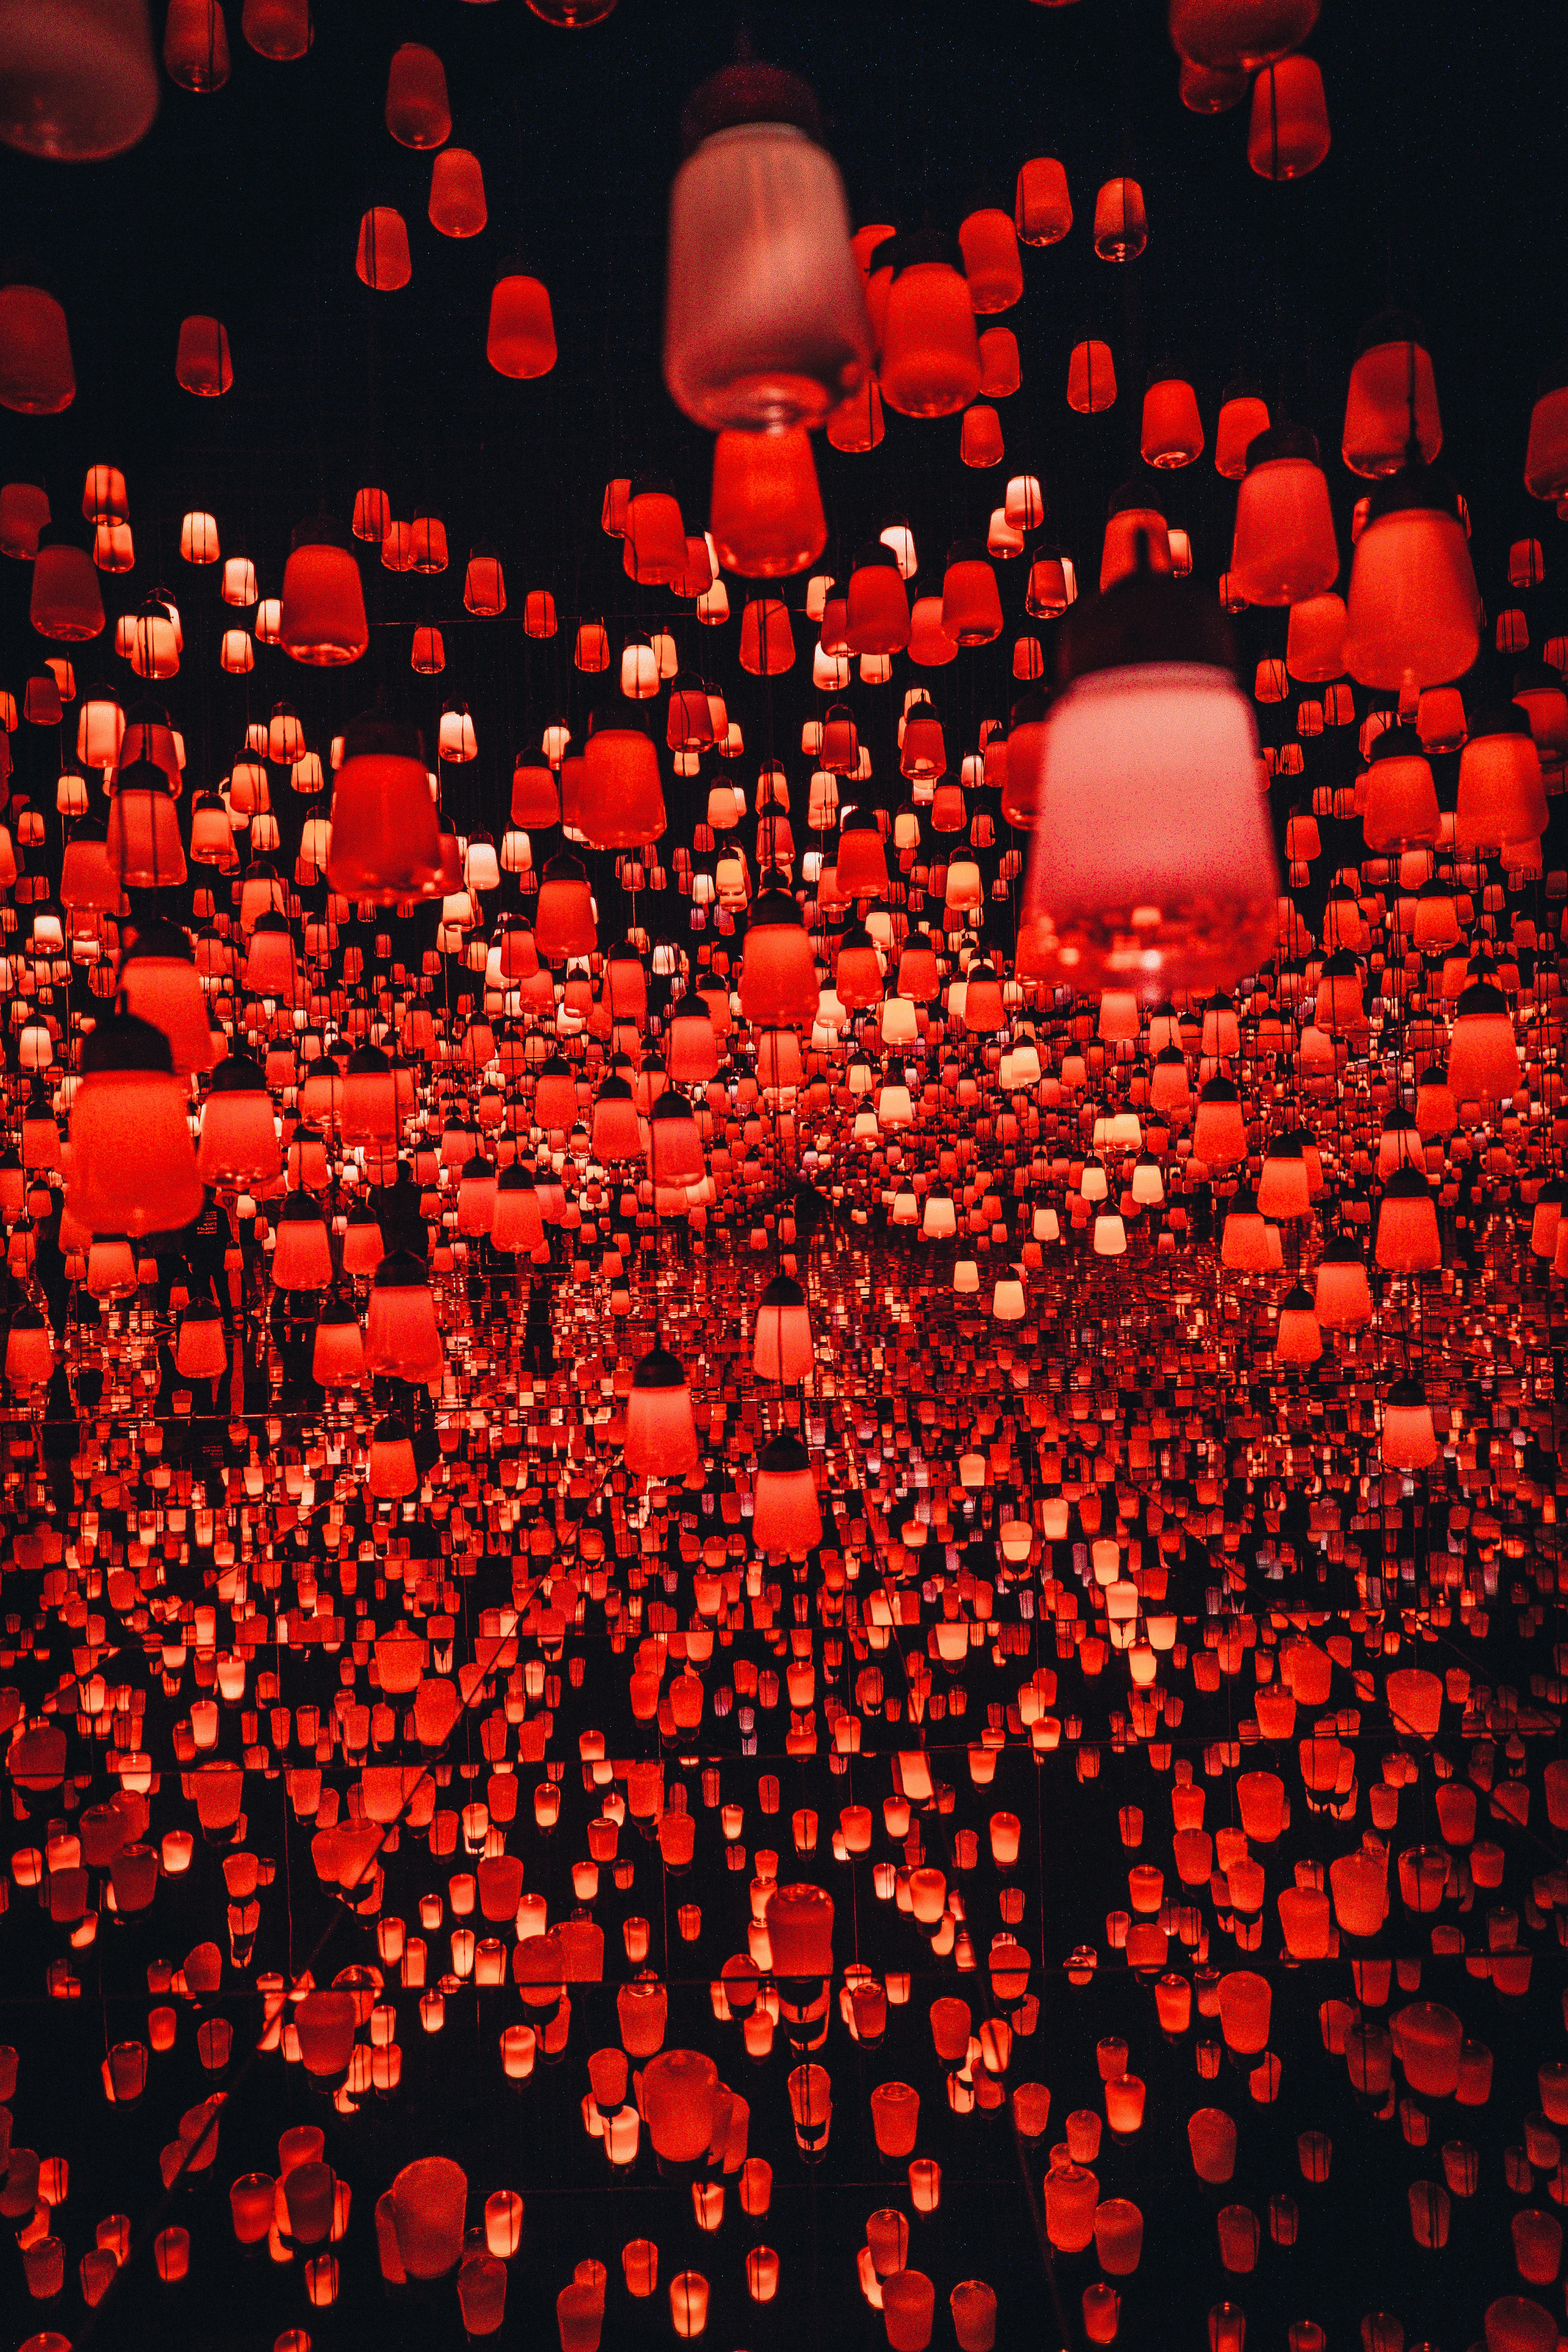
\includegraphics[width=6cm]{Figures/logo}}  %NEW: Changing logo
\def\extraspace{\vspace*{1.6cm}}
\makeatletter
\def\contactdetails{\faicon{phone} & \@telephone \\
                    \faicon{envelope} & \@email}
\makeatother

%%%% FRONT PAGE OF REPORTS

\def\reporttype{Report for}

\long\def\front#1#2#3{
\newpage
\begin{singlespacing}
\thispagestyle{empty}
\vspace*{-1.4cm}
\hspace*{-1.4cm}
\hbox to 16cm{
  \hbox to 6.5cm{\vbox to 14cm{\vbox to 25cm{
    \logo
    \vfill
    \parbox{6.3cm}{\raggedright
      \sf\color[rgb]{0.8, 0.7, 0.1 }    % NEW color 
      {\large\textbf{\name}}\par
      \vspace{.7cm}
      \tabcolsep=0.12cm\sf\small
      \begin{tabular}{@{}ll@{}}\contactdetails
      \end{tabular}
      \vspace*{0.3cm}\par
      ABN: \abn\par
    }
  }\vss}\hss}
  \hspace*{0.2cm}
  \hbox to 1cm{\vbox to 14cm{\rule{4pt}{26.8cm}\vss}\hss\hfill}  %NEW: Thicker line
  \hbox to 10cm{\vbox to 14cm{\vbox to 25cm{   
      \vspace*{3cm}\sf\raggedright
      \parbox{11cm}{\sf\raggedright\baselineskip=1.2cm
         \fontsize{24.88}{30}\color[rgb]{0, 0.29, 0.55}\sf\textbf{#1}}   % NEW: title color blue
      \par
      \vfill
      \large
      \vbox{\parskip=0.8cm #2}\par
      \vspace*{2cm}\par
      \reporttype\\[0.3cm]
      \hbox{#3}%\\[2cm]\
      \vspace*{1cm}
      {\large\sf\textbf{\Date~\Month~\Year}}
   }\vss}
  }}
\end{singlespacing}
\newpage
}

\makeatletter
\def\titlepage{\front{\expandafter{\@title}}{\@author}{\@organization}}
\makeatother

\usepackage{setspace}
\setstretch{1.5}

\usepackage{booktabs}
\usepackage{longtable}
\usepackage{array}
\usepackage{multirow}
\usepackage{wrapfig}
\usepackage{float}
\usepackage{colortbl}
\usepackage{pdflscape}
\usepackage{tabu}
\usepackage{threeparttable}
\usepackage{threeparttablex}
\usepackage[normalem]{ulem}
\usepackage{makecell}


\begin{document}
\titlepage

\clearpage

\hypertarget{introduction}{%
\section{Introduction}\label{introduction}}

The seatbelts dataset (\cite{seatbelts}) is a collection of monthly data from 1968 to 1984 collected by the Department of Transportation. The dataset includes data on number of deaths - for car drivers, front seat passengers, rear seat passengers and van drivers - as well as distance driven, petrol price and a dummy variable that denotes whether the law mandating that front seat passengers and drivers wear seatbelts was in effect. In this report, we aim to use this data to provide insight into the following questions

\begin{itemize}
\item
  \begin{enumerate}
  \def\labelenumi{\arabic{enumi})}
  \tightlist
  \item
    Did seatbelts have a notable effect on number of deaths?
  \end{enumerate}
\item
  \begin{enumerate}
  \def\labelenumi{\arabic{enumi})}
  \setcounter{enumi}{1}
  \tightlist
  \item
    Is there any relationship between driver deaths and the other variables in this dataset?
  \end{enumerate}
\item
  \begin{enumerate}
  \def\labelenumi{\arabic{enumi})}
  \setcounter{enumi}{2}
  \tightlist
  \item
    What is the trend and trough of driver deaths?
  \end{enumerate}
\item
  \begin{enumerate}
  \def\labelenumi{\arabic{enumi})}
  \setcounter{enumi}{3}
  \tightlist
  \item
    Is there any seasonality to number of deaths?
  \end{enumerate}
\end{itemize}

\hypertarget{compulsory-seatbelts-1983---alexi-tsakis}{%
\section{Compulsory Seatbelts 1983 - Alexi Tsakis}\label{compulsory-seatbelts-1983---alexi-tsakis}}

\begin{figure}
\centering
\includegraphics{report_files/figure-latex/DriversKilled-1.pdf}
\caption{\label{fig:DriversKilled}Drivers killed in accidents over time}
\end{figure}

\begin{figure}
\centering
\includegraphics{report_files/figure-latex/FrontKilled-1.pdf}
\caption{\label{fig:FrontKilled}Frontseat passengers killed in accidents over time}
\end{figure}

\begin{figure}
\centering
\includegraphics{report_files/figure-latex/RearKilled-1.pdf}
\caption{\label{fig:RearKilled}Backseat passengers killed in accidents over time}
\end{figure}

\begin{figure}
\centering
\includegraphics{report_files/figure-latex/VanKilled-1.pdf}
\caption{\label{fig:VanKilled}Light goods vehicle drivers killed in accidents over time}
\end{figure}

\begin{table}

\caption{\label{tab:DriverTable}Drivers killed before and after law}
\centering
\begin{tabular}[t]{r|r}
\hline
law & DriversKilled\_Average\\
\hline
0 & 125.8698\\
\hline
1 & 100.2609\\
\hline
\end{tabular}
\end{table}

\begin{table}

\caption{\label{tab:RearTable}Back seat passengers killed before and after law}
\centering
\begin{tabular}[t]{r|r}
\hline
law & Rear\_Average\\
\hline
0 & 400.3195\\
\hline
1 & 407.7391\\
\hline
\end{tabular}
\end{table}

\begin{table}

\caption{\label{tab:FrontTable}Front seat passengers killed before and after law}
\centering
\begin{tabular}[t]{r|r}
\hline
law & Front\_Average\\
\hline
0 & 873.4556\\
\hline
1 & 570.9565\\
\hline
\end{tabular}
\end{table}

\begin{table}

\caption{\label{tab:VanTable}Light good vehicle drivers killed before and after law}
\centering
\begin{tabular}[t]{r|r}
\hline
law & Van\_Average\\
\hline
0 & 9.585799\\
\hline
1 & 5.173913\\
\hline
\end{tabular}
\end{table}

In this section we look at the effect of seatbelts on driver deaths in the UK. Front seatbelts were compulsory on all new cars registered in the UK from 1968, however it was not required for them to be worn until 1983. In this section, we will answer the question - did mandatory wearing of frontrow seatbelts prevent deaths for drivers and passengers?

First, to answer if any relationships shown are causation and not simply correlation, we ask - why do seatbelts prevent deaths? According to the National Highway Traffic Safety Administration, the primary reasons why seatbelts prevent death is that ``Buckling up helps keep you safe and secure inside your vehicle, whereas not buckling up can result in being totally ejected from the vehicle in a crash, which is almost always deadly.'' (\cite{NHTSA})

These scenarios are referred to as ``secondary collisions'' - i.e.~a crash event that results from the impact of an initial collison, such as ejection from a vehicle, or even a high speed impact with objects inside the vehicle.

Now that we understand the theory behind the impact of seatbelts on preventing death, let us look at the data:

There is a clear negative correlation between frontrow passengers and light good vehicle drivers killed since the introduction of the law (figure \ref{fig:FrontKilled}, figure \ref{fig:VanKilled}), data from the introduction of the law shown in blue).

There is also a clear reduction in number of drivers killed (figure \ref{fig:DriversKilled}) since the introduction of compulsory seatbelts - the lack of change since the introduction of the law, but the large change since approximately 1973 can be described as " drivers that are least likely to use seat belts might be those that are more likely to be involved in an accident" (\cite{Cohen}) - i.e.~that careful drivers adopted seatbelts already without the law, and those likely to get involved in accidents would be unlikely to wear seatbelts even with the law in place.

There is little change in number of rear seat passengers killed (figure \ref{fig:RearKilled}) - this is because the regulations and law were only for front seat seatbelts, and not backseat seatbelts, suggesting the total number of accidents didn't change.

We can also see this in tabular format, so it is easier to see the effect of the law numerically (table \ref{tab:DriverTable}, table \ref{tab:RearTable}, table \ref{tab:FrontTable}, table \ref{tab:VanTable}).

\clearpage

\hypertarget{reseach-questions---siyi-li}{%
\section{Reseach Questions - Siyi Li}\label{reseach-questions---siyi-li}}

\begin{itemize}
\item
  Is there any relationship between the DriversKilled variable and other variables?
\item
  Can we build an model among these variables?
\end{itemize}

\hypertarget{analysis}{%
\section{Analysis}\label{analysis}}

\hypertarget{is-there-any-relationship-between-the-driverskilled-variable-and-other-variables}{%
\subsection{Is there any relationship between the DriversKilled variable and other variables?}\label{is-there-any-relationship-between-the-driverskilled-variable-and-other-variables}}

\begin{table}

\caption{\label{tab:mytables}Summary of the three variabls}
\centering
\begin{tabular}[t]{l|l|l|l}
\hline
  & DriversKilled &    drivers &     front\\
\hline
 & Min.   : 60.0 & Min.   :1057 & Min.   : 426.0\\
\hline
 & 1st Qu.:104.8 & 1st Qu.:1462 & 1st Qu.: 715.5\\
\hline
 & Median :118.5 & Median :1631 & Median : 828.5\\
\hline
 & Mean   :122.8 & Mean   :1670 & Mean   : 837.2\\
\hline
 & 3rd Qu.:138.0 & 3rd Qu.:1851 & 3rd Qu.: 950.8\\
\hline
 & Max.   :198.0 & Max.   :2654 & Max.   :1299.0\\
\hline
\end{tabular}
\end{table}

From the table \ref{tab:mytables} shows:

\begin{itemize}
\item
  the minimum number of drivers killed is 60 and the maximum is 198.
\item
  the minimum number of drivers is 1057 and the maximum is 2654.
\item
  the minimum number of front-seat passengers killed or seriously injured is 426 and the maximum is 1299.
\item
  when the number of the drivers increase, the number of the drivers killed also increase. Therefore, I guess there is a positive relationship between the variable drivers and the variable drivers killed.
\end{itemize}

In order to develop the relationship between the number of drivers and car drivers killed, we can use GGally package (\cite{10}) to produce the correlation graph.

\begin{figure}[H]

{\centering \includegraphics{report_files/figure-latex/myggpair-1} 

}

\caption{Correlation between variables}\label{fig:myggpair}
\end{figure}

\begin{itemize}
\item
  The figure \ref{fig:myggpair} shows that there are positive relationships between drivers variable and Driverskilled variable, front variable and Driverskilled variable, VanKilled and Driverskilled, rear variable and Driverskilled variable. Especially, we can see that the variables of front and drivers are highly positive related to the Driverskilled variable since the correlations between that are 0.707 and 0.889 respectively.
\item
  It also indicates that the relationships between kms and Driverskilled variable, PetrolPrice and Driverskilled, and law and Driverskilled are negative.
\item
  In fact, there are some correlations between each pair of variables but i just focus on the relationship between the response variable Driverskiied and other predictor.
\end{itemize}

\hypertarget{can-we-build-an-model-among-these-variables}{%
\subsection{Can we build an model among these variables?}\label{can-we-build-an-model-among-these-variables}}

\begin{verbatim}
## 
## Call:
## lm(formula = DriversKilled ~ ., data = Seatbelt)
## 
## Residuals:
##     Min      1Q  Median      3Q     Max 
## -29.489  -7.620  -0.531   7.676  34.700 
## 
## Coefficients:
##               Estimate Std. Error t value Pr(>|t|)    
## (Intercept) -2.330e+01  1.472e+01  -1.583    0.115    
## drivers      8.327e-02  5.544e-03  15.018   <2e-16 ***
## front       -3.838e-03  1.723e-02  -0.223    0.824    
## rear         5.189e-03  2.474e-02   0.210    0.834    
## kms          5.875e-04  5.025e-04   1.169    0.244    
## PetrolPrice -1.629e+01  8.643e+01  -0.188    0.851    
## VanKilled    5.928e-02  2.911e-01   0.204    0.839    
## law1         4.070e+00  4.076e+00   0.998    0.319    
## ---
## Signif. codes:  0 '***' 0.001 '**' 0.01 '*' 0.05 '.' 0.1 ' ' 1
## 
## Residual standard error: 11.58 on 184 degrees of freedom
## Multiple R-squared:  0.7993, Adjusted R-squared:  0.7917 
## F-statistic: 104.7 on 7 and 184 DF,  p-value: < 2.2e-16
\end{verbatim}

The linear model shows that just the drivers variable are significant which means that the drivers are fit the model. Other variables include the Intercept are not significant since their p-value are larger than 0.05, which means that the model can not fit all the variables very well.

\clearpage

\begin{figure}
\centering
\includegraphics{report_files/figure-latex/residuals-1.pdf}
\caption{\label{fig:residuals}residuals VS fitted value}
\end{figure}

In order to analyze the residuals, I use the \textbf{broom} package(\cite{11}).

From the figure \ref{fig:residuals}, it indicates that the residuals does not include obvious pattern of the variables since the residuals are randomly around the red line. It means that the model can capture most information about the response variable DriversKilled. But we can see that the tail at the beginning and end is not like a straight since the observations are not enough at the end and the beginning.

\hypertarget{research-questions---yusen-wang}{%
\section{Research Questions - Yusen Wang}\label{research-questions---yusen-wang}}

\begin{itemize}
\item
  From the data on the number of driver deaths, which time period was the peak, and what historical facts accompany the change after the peak ? How about the trend before and after law introduced ?
\item
  Is there any relationship between season and driverskilled?
\end{itemize}

\hypertarget{data-analysis}{%
\section{Data Analysis}\label{data-analysis}}

\hypertarget{analysis-of-trends-in-driverkilled-before-and-after-1983}{%
\subsection{Analysis of trends in driverkilled before and after 1983}\label{analysis-of-trends-in-driverkilled-before-and-after-1983}}

\begin{figure}
\centering
\includegraphics{report_files/figure-latex/figureE-1.pdf}
\caption{\label{fig:figureE}Trend Lines}
\end{figure}

According to Figure \ref{fig:figureE}, as we can see:

\begin{itemize}
\tightlist
\item
  the trend line of DriversKilled and FrontDeath after 1970 began to decline.
\end{itemize}

The reason is Successive UK governments proposed, but failed to deliver, seat belt legislation throughout the 1970s. Front seat belts were compulsory equipment on all new cars registered in the UK from 1968, although it did not become compulsory for them to be worn until 1983. (\cite{richens2000condoms}) \clearpage

\begin{figure}
\centering
\includegraphics{report_files/figure-latex/Bluebox-1.pdf}
\caption{\label{fig:Bluebox}Law Introduction}
\end{figure}

From the figure \ref{fig:Bluebox}, it is clear that the range of monthly deaths among drivers before the law was higher than after it was enacted.

\begin{table}

\caption{\label{tab:Beforelawsub}Before Law summary stats}
\centering
\begin{tabular}[t]{l|l|l|l|l|l|l|l|l|l|l}
\hline
  &      Year &     Month & DriversKilled &    drivers &     front &      rear &      kms &  PetrolPrice &   VanKilled &      law\\
\hline
 & Min.   :1969 & Jan    :15 & Min.   : 79.0 & Min.   :1309 & Min.   : 567.0 & Min.   :224.0 & Min.   : 7685 & Min.   :0.08118 & Min.   : 2.000 & Min.   :0\\
\hline
 & 1st Qu.:1972 & Feb    :14 & 1st Qu.:108.0 & 1st Qu.:1511 & 1st Qu.: 767.0 & 1st Qu.:344.0 & 1st Qu.:12387 & 1st Qu.:0.09078 & 1st Qu.: 7.000 & 1st Qu.:0\\
\hline
 & Median :1976 & Mar    :14 & Median :121.0 & Median :1653 & Median : 860.0 & Median :401.0 & Median :14455 & Median :0.10273 & Median :10.000 & Median :0\\
\hline
 & Mean   :1976 & Apr    :14 & Mean   :125.9 & Mean   :1718 & Mean   : 873.5 & Mean   :400.3 & Mean   :14463 & Mean   :0.10187 & Mean   : 9.586 & Mean   :0\\
\hline
 & 3rd Qu.:1979 & May    :14 & 3rd Qu.:140.0 & 3rd Qu.:1926 & 3rd Qu.: 986.0 & 3rd Qu.:454.0 & 3rd Qu.:16585 & 3rd Qu.:0.11132 & 3rd Qu.:13.000 & 3rd Qu.:0\\
\hline
 & Max.   :1983 & Jun    :14 & Max.   :198.0 & Max.   :2654 & Max.   :1299.0 & Max.   :646.0 & Max.   :21040 & Max.   :0.13303 & Max.   :17.000 & Max.   :0\\
\hline
 & NA & (Other):84 & NA & NA & NA & NA & NA & NA & NA & NA\\
\hline
\end{tabular}
\end{table}

\begin{table}

\caption{\label{tab:Afterlawsub}After Law summary stats}
\centering
\begin{tabular}[t]{l|l|l|l|l|l|l|l|l|l|l}
\hline
  &      Year &     Month & DriversKilled &    drivers &     front &      rear &      kms &  PetrolPrice &   VanKilled &      law\\
\hline
 & Min.   :1983 & Feb    : 2 & Min.   : 60.0 & Min.   :1057 & Min.   :426.0 & Min.   :296.0 & Min.   :15511 & Min.   :0.1131 & Min.   :2.000 & Min.   :1\\
\hline
 & 1st Qu.:1983 & Mar    : 2 & 1st Qu.: 85.0 & 1st Qu.:1171 & 1st Qu.:516.0 & 1st Qu.:347.0 & 1st Qu.:17971 & 1st Qu.:0.1148 & 1st Qu.:3.500 & 1st Qu.:1\\
\hline
 & Median :1984 & Apr    : 2 & Median : 92.0 & Median :1282 & Median :585.0 & Median :408.0 & Median :19162 & Median :0.1161 & Median :5.000 & Median :1\\
\hline
 & Mean   :1984 & May    : 2 & Mean   :100.3 & Mean   :1322 & Mean   :571.0 & Mean   :407.7 & Mean   :18890 & Mean   :0.1165 & Mean   :5.174 & Mean   :1\\
\hline
 & 3rd Qu.:1984 & Jun    : 2 & 3rd Qu.:119.0 & 3rd Qu.:1464 & 3rd Qu.:629.5 & 3rd Qu.:471.5 & 3rd Qu.:19952 & 3rd Qu.:0.1180 & 3rd Qu.:7.000 & 3rd Qu.:1\\
\hline
 & Max.   :1984 & Jul    : 2 & Max.   :154.0 & Max.   :1763 & Max.   :721.0 & Max.   :521.0 & Max.   :21626 & Max.   :0.1201 & Max.   :8.000 & Max.   :1\\
\hline
 & NA & (Other):11 & NA & NA & NA & NA & NA & NA & NA & NA\\
\hline
\end{tabular}
\end{table}

From the tables \ref{tab:Beforelawsub} and \ref{tab:Afterlawsub} :

\begin{itemize}
\item
  Before law introduced, the median of DriversKilled is 121, the minimum number is 79 and the maximum number is 198.
\item
  After introduced, the median of DriversKilled is 92, the minimum number is 60 and the maximum number is 154.
\end{itemize}

We can see that the law is effective in helping drivers stay away from death, since it is introduced on 31st January 1983.

\begin{figure}
\centering
\includegraphics{report_files/figure-latex/season-1.pdf}
\caption{\label{fig:season}Seasonality}
\end{figure}

From the figure \ref{fig:season}, there seems to be some seasonal correlation between driver deaths:

\begin{itemize}
\item
  it is quite obvious that, there is more driver deaths and front deaths in autumn/winter than in spring/summer, somehow it is with seasonal effect. Snow, rain, fog, and other bad weather is the main reason, not only affect the driver's vision, but also increase the braking distance.
\item
  based on the color plots, it can be seem that the number of driver deaths is the lowest after the front seatbelt legislation been introduced.
\end{itemize}

\hypertarget{conclusion}{%
\section{Conclusion}\label{conclusion}}

Based on the analysis done in this report, our findings were as follows

\begin{itemize}
\tightlist
\item
  The mandatory seatbelt production law of 1968, as well as the mandatory seatbelt wearing law of 1983 did have a statistically significant impact in reducing number of drivers, van drivers and front seat passengers killed. The laws slightly increased number of rear seat passengers killed, but not significantly so.
\item
  There is no statistically significant relationship between DriversKilled and any other variable in the dataset except number of drivers, as such we can't model DriversKilled very well as Drivers does not explain enough of the variance.
\item
  The trough of drivers killed is after the seatbelt legislation was introduced.
\item
  There is more deaths in autumn and winter due to weather conditions.
\end{itemize}

\begin{center}\rule{0.5\linewidth}{0.5pt}\end{center}

\hypertarget{packages-used}{%
\section{Packages used}\label{packages-used}}

\cite{1}
\cite{2}
\cite{3}
\cite{4}
\cite{9}

\printbibliography

\end{document}
